\subsection{The Muon Spectrometer}
\label{sec:ms}

Surrounding the calorimeters is the muon spectrometer (MS)~\cite{CERN-LHCC-97-022}, responsible
for the detection of high-momentum muons originating from the $pp$ interaction.
The MS is based on the magnetic deflection of muon tracks, allowing for their
momentum determination.
The bending of the muon trajectories is provided by the large
superconducting air-core toroid magnet system, illustrated in Figure~\ref{fig:atlas_magnet_system},
consisting of a large barrel toroid over the range $\lvert \eta \rvert < 1.4$
and end-cap toroid systems in the range $1.6 < \lvert \eta \rvert < 2.7$.
The superconducting toroid magnet provides an average field of $4\,$T.
The magnetic field bending strength is roughly constant in $\eta$, except in the
region in which the transition between the barrel and end-cap toroids takes place
($1.4 < \lvert \eta \rvert < 1.6$).
It should be noted that the overall design of the superconducting toroid structure,
dictated by the requirements of the MS, is what gives ATLAS its large size and essentially
drove the original design of all subdetectors discussed in previous sections.
A view of the ATLAS detector is shown in Figure~\ref{fig:atlas_in_cavern},
where it can be seen that the volume enclosed by the MS takes up most of free volume
in the underground experimental cavern at Point 1.
Four types of gaseous radiation detector are used in the MS.
They can be categorized as being either \textit{precision} or \textit{trigger} chambers.
A view of the MS, highlighting layout of its detectors, is shown in Figure~\ref{fig:muon_plan_view_eta}.

\begin{figure}[!htb]
    \begin{center}
        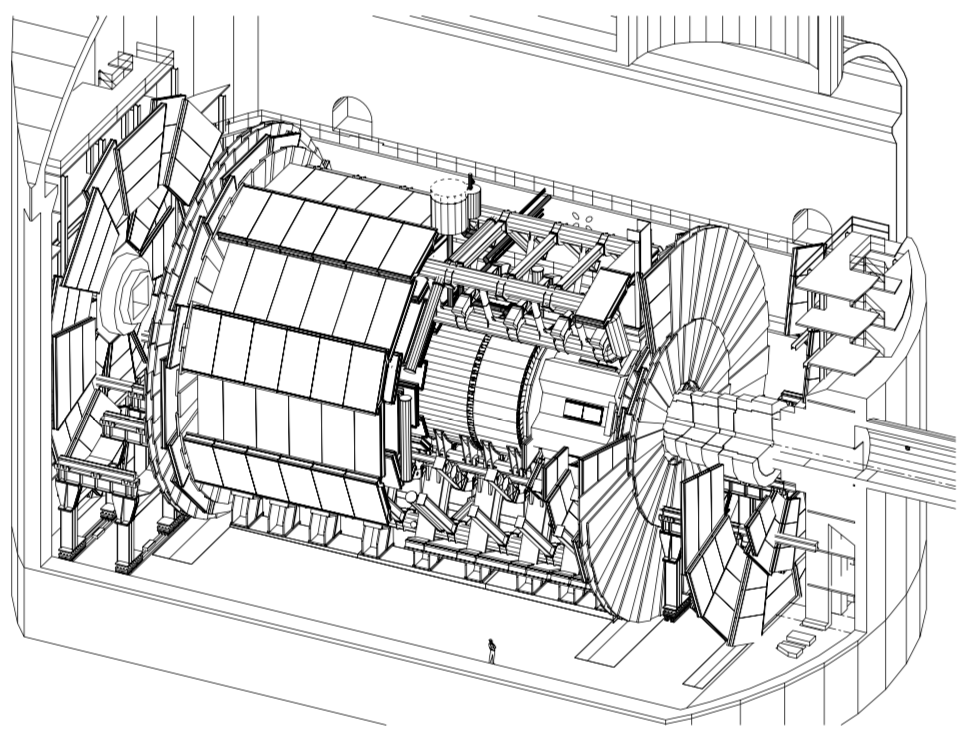
\includegraphics[width=0.8\textwidth]{figures/chapter2/atlas_in_cavern}
        \caption{
            A view of the ATLAS detector inside the underground experimental area
            UX15.
            Notice that the outermost muon stations in the forward regions are located
            at the extreme ends of the cavern.
            {\color{red}{Should move this figure either above or entirely}}
        }
        \label{fig:atlas_in_cavern}
    \end{center}
\end{figure}

\begin{figure}[!htb]
    \begin{center}
        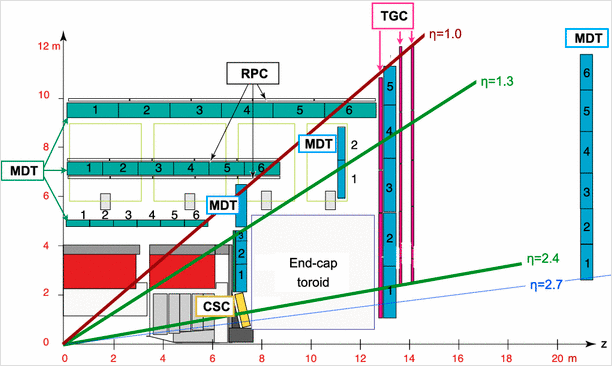
\includegraphics[width=0.8\textwidth]{figures/chapter2/muon_spec/atlas_muon_plan_view_eta}
        \caption{
            A view in the $r-z$ plane of a quadrant of the muon spectrometer (MS).
            Indicated by color are the four detector technologies used in the MS:
            MDT (blue), RPC (grey), TGC (red), and CSC (yellow).
            The light grey boxes at $6 < r < 9$\,m indicate the location of the
            barrel toroid structures.
            Also shown are the envelopes in $\lvert \eta \rvert$ of the barrel,
            small wheel, and big wheel sections of the MS.
        }
        \label{fig:muon_plan_view_eta}
    \end{center}
\end{figure}
\FloatBarrier

\begin{figure}[!htb]
    \begin{center}
        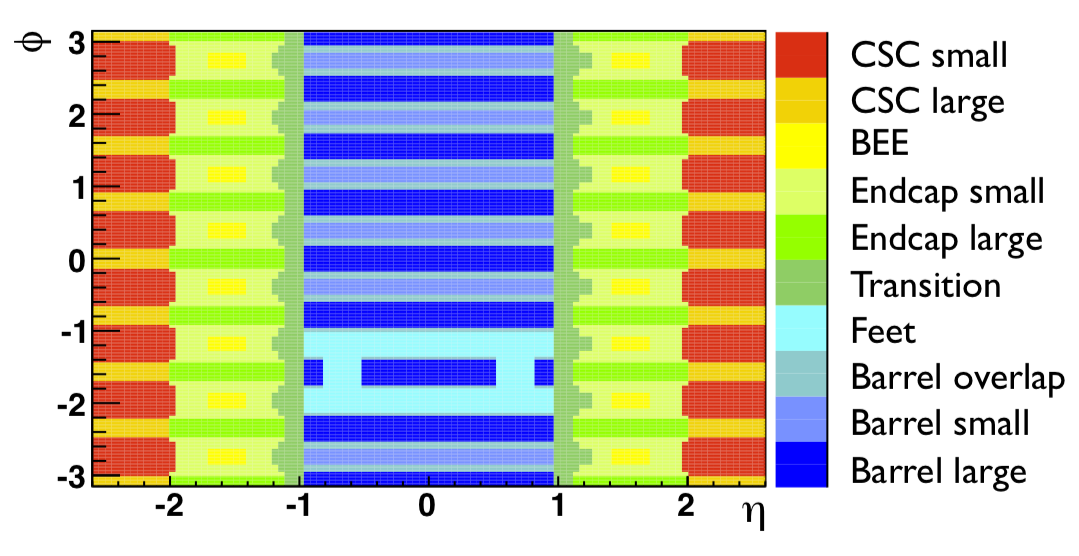
\includegraphics[width=0.7\textwidth]{figures/chapter2/muon_spec/atlas_muon_overlap}
        \caption{
        }
        \label{fig:muon_overlap}
    \end{center}
\end{figure}

\begin{figure}[!htb]
    \begin{center}
        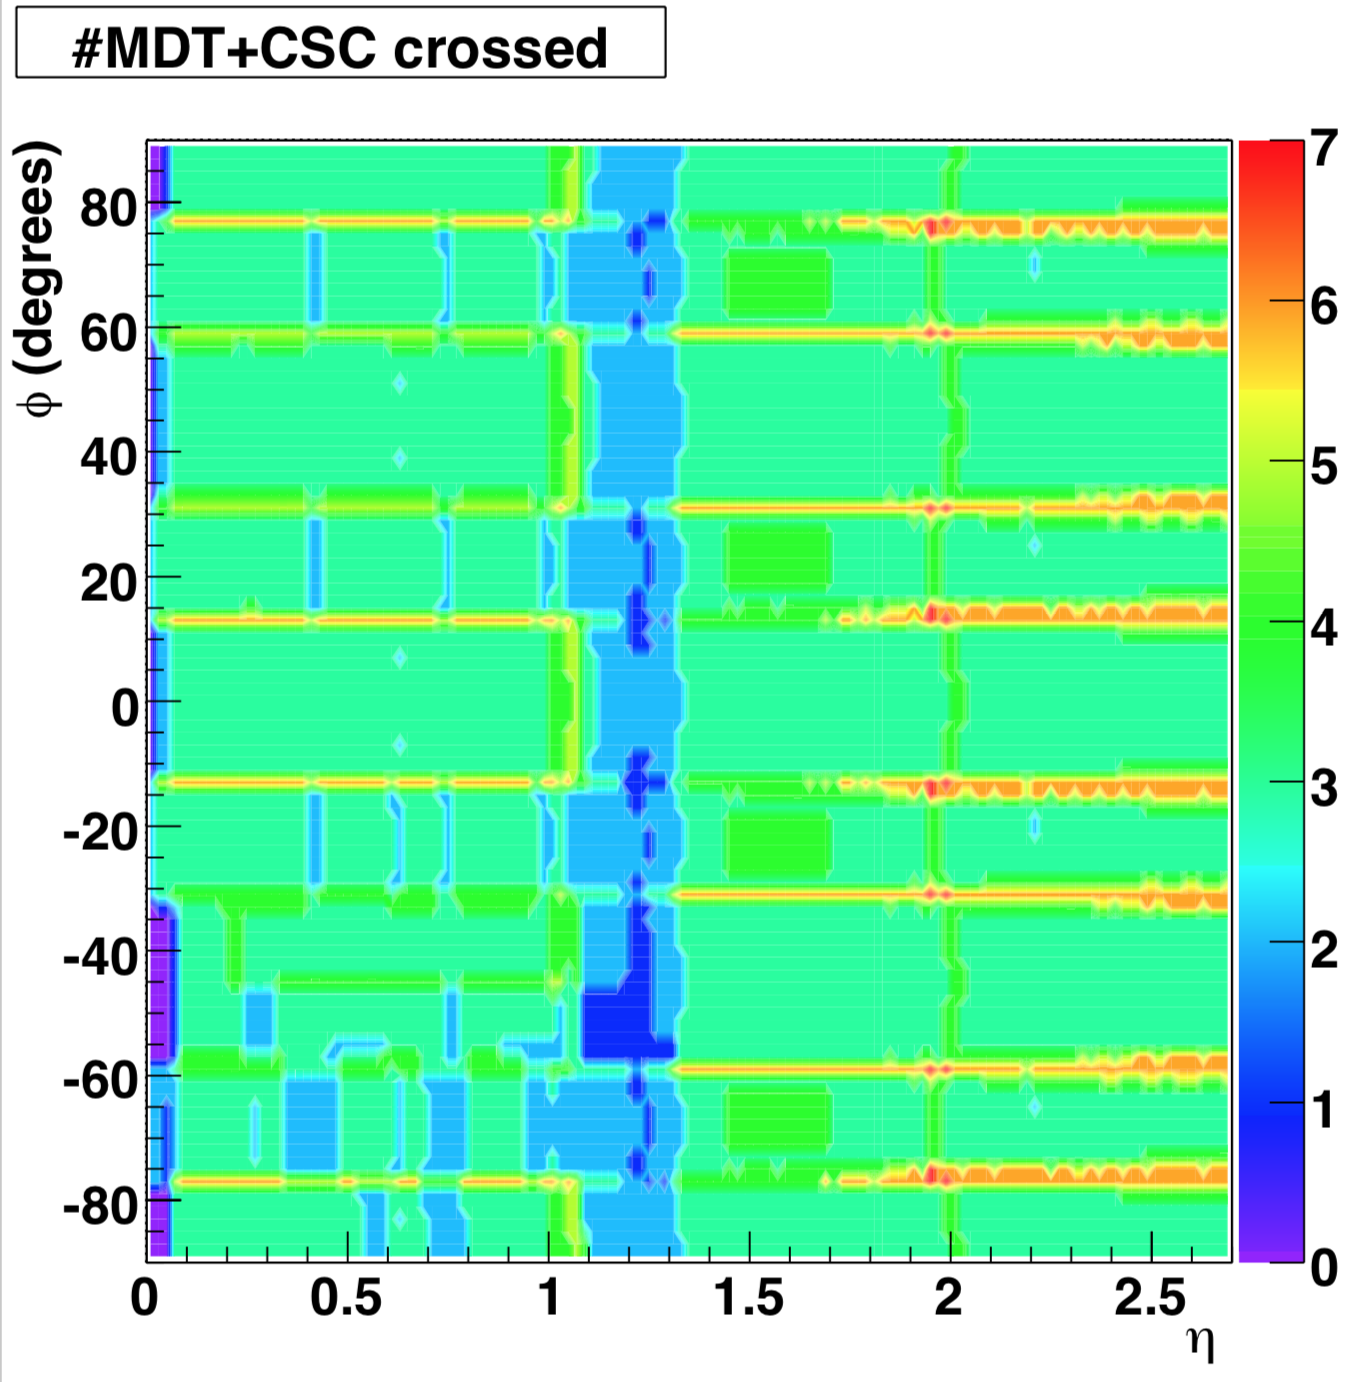
\includegraphics[width=0.7\textwidth]{figures/chapter2/muon_spec/atlas_ms_nchamber_crossed}
        \caption{
        }
        \label{fig:muon_nchambers_crossed}
    \end{center}
\end{figure}


\subsubsection{Precision Muon Chambers}
\label{sec:muon_precision}

\begin{figure}[!htb]
    \begin{center}
        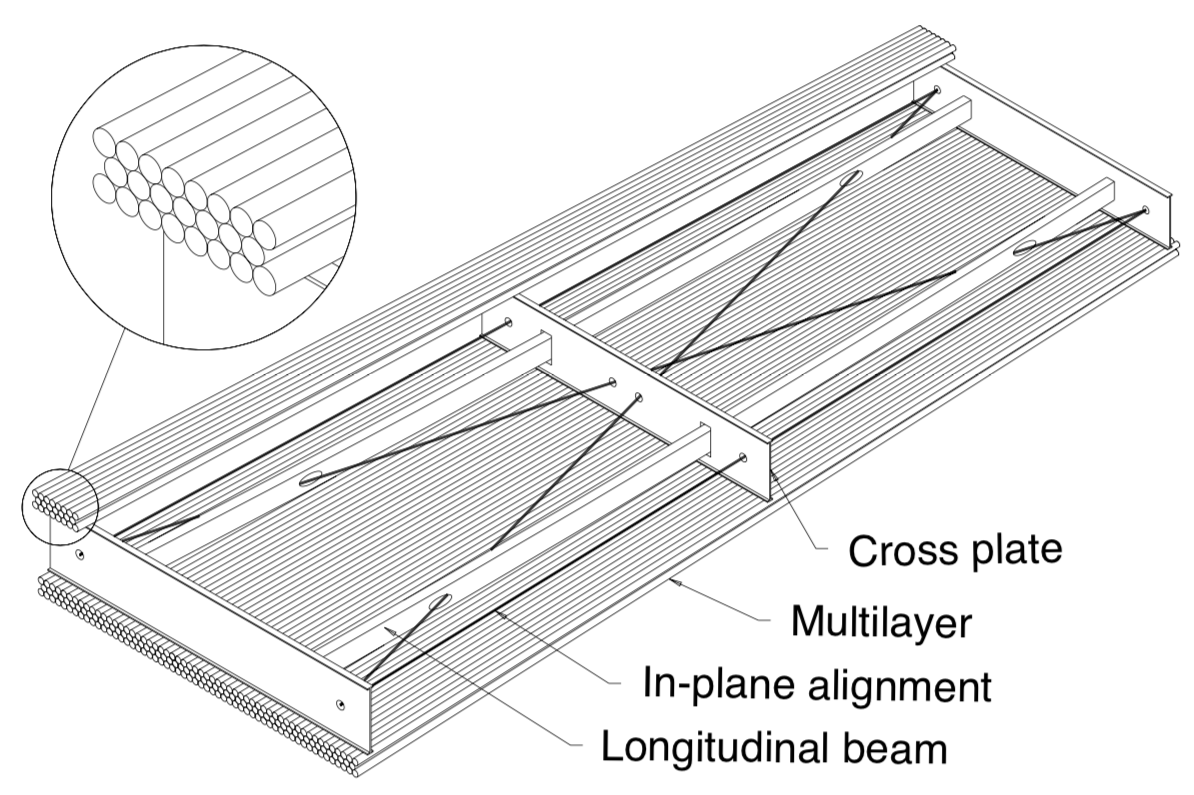
\includegraphics[width=0.5\textwidth]{figures/chapter2/muon_spec/mdt_chamber}
        \raisebox{1.22cm}{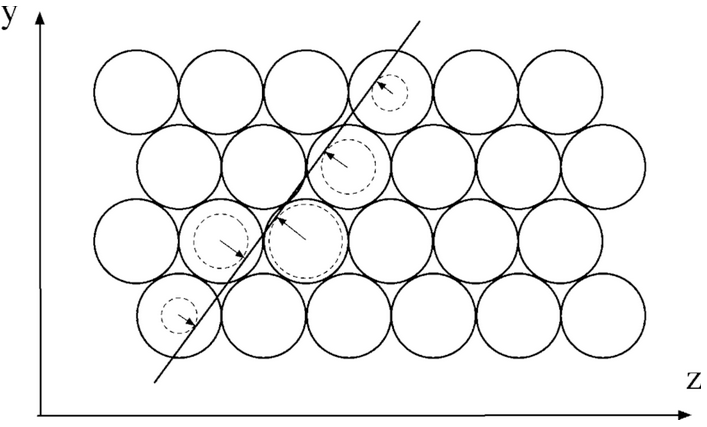
\includegraphics[width=0.32\textwidth]{figures/chapter2/muon_spec/mdt_trackfit}}
        \caption{
            \textit{Left}: Illustration of a double-multilayer MDT chamber with its internal alignment
                and support structure exposed. A zoom-in on the multilayer of MDT tubes is shown.
            \textit{Right}: Illustration of the multilayer MDT tracklet-fitting algorithm~\cite{MDTtrackfit}.
        }
        \label{fig:mdt_chamber}
    \end{center}
\end{figure}

\begin{figure}[!htb]
    \begin{center}
        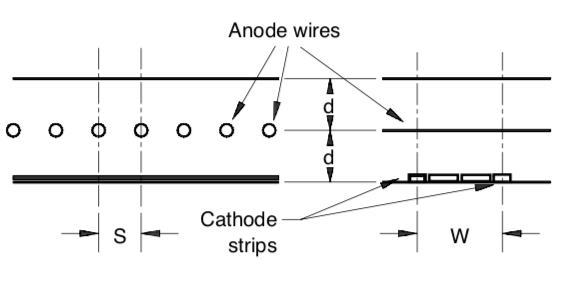
\includegraphics[width=0.55\textwidth]{figures/chapter2/muon_spec/csc_chamber}
        \caption{
            Diagram showing the main components of a cathode-strip chamber (CSC).
            On the \textit{left} (\textit{right}) is a view parallel (perpendicular) to the anode
            wires and perpendicular (parallel) to the cathode strips.
        }
        \label{fig:csc_chamber}
    \end{center}
\end{figure}

\subsubsection{Muon Trigger Chambers}
\label{sec:muon_trigger}

\begin{figure}[!htb]
    \begin{center}
        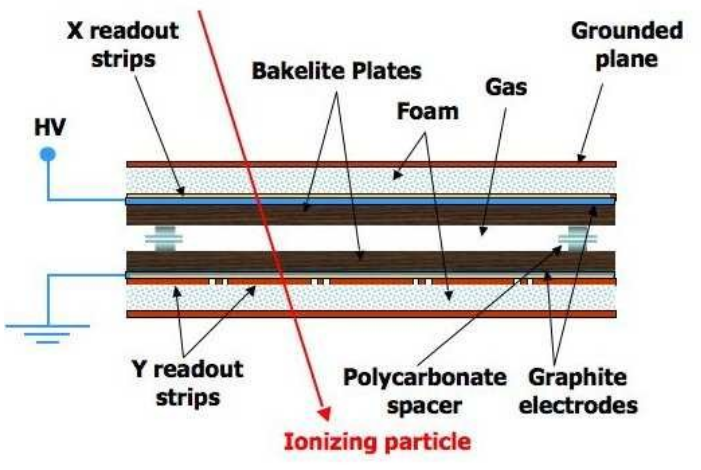
\includegraphics[width=0.5\textwidth]{figures/chapter2/muon_spec/rpc_chamber}
        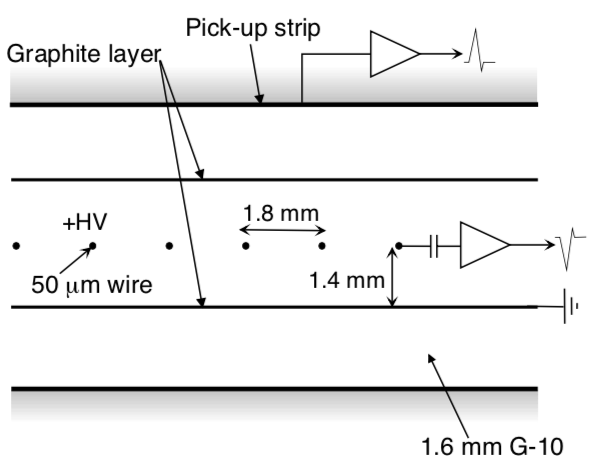
\includegraphics[width=0.38\textwidth]{figures/chapter2/muon_spec/tgc_chamber}
        \caption{
            \textit{Left}: Illustration of a resistive plate chamber (RPC) and its principle of operation.
            \textit{Right}: Diagram showing the main components of a thin-gap chamber (TGC).
        }
        \label{fig:muon_trigger_chamber}
    \end{center}
\end{figure}
